% -*- coding: UTF-8 -*-
% hello.tex

\documentclass[UTF8,oneside]{ctexbook}

% \usepackage{xeCJK}
\usepackage[utf8]{inputenc}

% load paralist before enumitem
\usepackage{paralist}

\usepackage{hyperref}
\hypersetup{pdftex,colorlinks=true,allcolors=blue}
\usepackage{hypcap}

\usepackage{color}
\usepackage[usenames, dvipsnames, svgnames, table]{xcolor}
% \pagecolor{gray}

\usepackage{makeidx}
\makeindex

\usepackage{amsmath}
\usepackage{mathtools}

\usepackage{listings}
\usepackage{multicol}
\usepackage{fancybox}
\usepackage{tcolorbox}
\usepackage{enumitem}

\usepackage{indentfirst}

\newenvironment{enumbox}[0]{
    \begin{tcolorbox}
    \begin{compactenum}
} {
    \end{compactenum}
    \end{tcolorbox}
}

\newenvironment{itembox}[0]{
    \begin{tcolorbox}
    \begin{compactitem}
} {
    \end{compactitem}
    \end{tcolorbox}
}

% table
\setlength{\arrayrulewidth}{1pt}
\setlength{\tabcolsep}{16pt}
\renewcommand{\arraystretch}{2.5}
\newcolumntype{s}{>{\columncolor[HTML]{AAACED}} p{3cm}}

\arrayrulecolor[HTML]{DB5800}

\usepackage{tikz,mathpazo}
\usetikzlibrary{positioning, fit, matrix, shapes, arrows, chains, trees, arrows.meta}

% \bibliographystyle{plain}
% \bibliography{math}

\tikzset{%
  >={Latex[width=2mm,length=2mm]},
  % Specifications for style of nodes:
            base/.style = {rectangle, rounded corners, draw=black,
                           minimum width=4cm, minimum height=1cm,
                           text centered, font=\sffamily},
  activityStarts/.style = {base, fill=blue!30},
       startstop/.style = {base, fill=red!30},
    activityRuns/.style = {base, fill=green!30},
         process/.style = {base, minimum width=2.5cm, fill=orange!15,
                           font=\ttfamily},
}

% 摘录
\usepackage{verbatim}
\usepackage{libertine}
\usepackage{graphicx}
\usepackage{framed}

\newcommand*\openquote{\makebox(25,-22){\scalebox{5}{``}}}
\newcommand*\closequote{\makebox(25,-22){\scalebox{5}{''}}}
\colorlet{shadecolor}{Azure}

\makeatletter
\newif\if@right
\def\shadequote{\@righttrue\shadequote@i}
\def\shadequote@i{\begin{snugshade}\begin{quote}\openquote}
\def\endshadequote{%
\if@right\hfill\fi\closequote\end{quote}\end{snugshade}}
\@namedef{shadequote*}{\@rightfalse\shadequote@i}
\@namedef{endshadequote*}{\endshadequote}
\makeatother

\usepackage[normalem]{ulem}

\newcommand{\hl}{\bgroup\markoverwith
  {\textcolor{yellow}{\rule[-.5ex]{2pt}{2.5ex}}}\ULon}

%\usepackage{soul}

%\newcommand{\hlc}[2][yellow]{{%
%    \colorlet{foo}{#1}%
%    \sethlcolor{foo}\hl{#2}}%
%}

% todonode
\usepackage{lipsum}                     % Dummytext
\usepackage{xargs}                      % Use more than one optional parameter in a new commands
% 
\usepackage[colorinlistoftodos,prependcaption,textsize=tiny]{todonotes}
\newcommandx{\unsure}[2][1=]{\todo[linecolor=red,backgroundcolor=red!25,bordercolor=red,#1]{#2}}
\newcommandx{\change}[2][1=]{\todo[linecolor=blue,backgroundcolor=blue!25,bordercolor=blue,#1]{#2}}
\newcommandx{\info}[2][1=]{\todo[linecolor=OliveGreen,backgroundcolor=OliveGreen!25,bordercolor=OliveGreen,#1]{#2}}
\newcommandx{\improvement}[2][1=]{\todo[linecolor=Plum,backgroundcolor=Plum!25,bordercolor=Plum,#1]{#2}}
\newcommandx{\thiswillnotshow}[2][1=]{\todo[disable,#1]{#2}}
%

\usepackage[simplified]{pgf-umlcd}

\title{SUZAKU架构文档}
\author{董冠军}
\date{\today}

\begin{document}

\maketitle
\tableofcontents

\listoftodos[Notes]

\part{架构}

\chapter{架构}

\section{RAID分析}

RAID分析作为架构驱动力

假设和信念
\begin{enumbox}
\item 云是新常态
\item 数据资产是战略资源
\item 全闪是大势所趋
\end{enumbox}

新设计解决了什么老问题?
\begin{enumbox}
\item 单卷的水平扩展问题
\item IO path上的数据转发问题
\item allocate性能低,影响精简配置和COW性能
\item 每个节点导出core、disk等资源,进行全局调度(均衡)
\item 灵活的MM
\item thread local影响CPU利用率
\item ***
\item 重新调整数据布局
\item 单卷大小的限制(支持大卷)
\item chkinfo是动态大小的,副本数、EC配置
\item 底层chunk对象依然不是跨卷的
\item ***
\item COW: volume和snapshot共享对象
\item ***
\item table1/table2实现过于复杂的问题
\item disk md and slots
\item coroutine难于调试
\item ***
\item 多网络
\item MULTIPATH
\item IPv6
\end{enumbox}

\section{模块}

分布式系统架构通常包括几个部分:client、mds、cds。分别对应什么?
\begin{center}
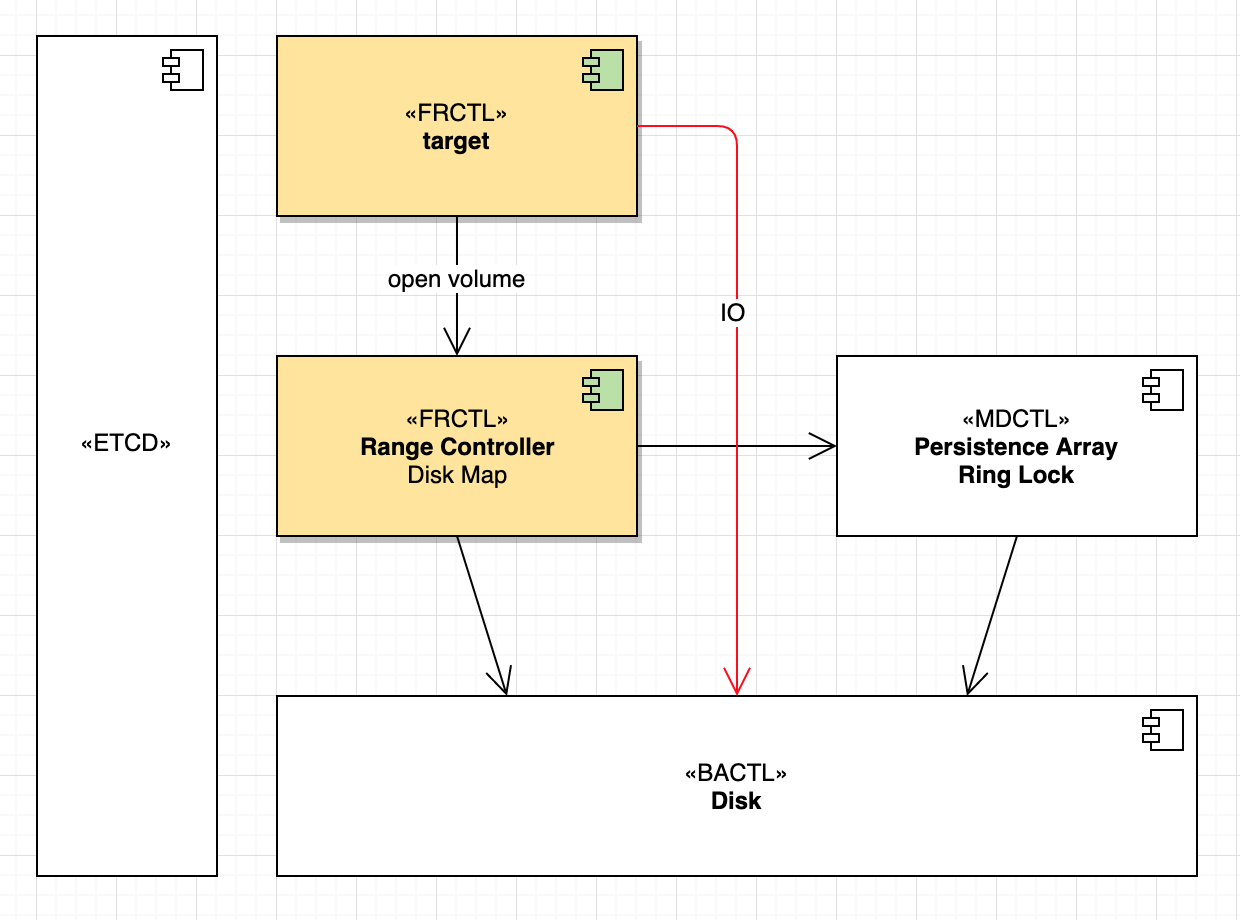
\includegraphics[width=11cm]{../imgs/modules.png}
\end{center}

target到bactl,有两条路径,视是否通过range ctl而定。如果不通过range ctl(rangectl bypass),数据流可直达后端存储,
实现控制流和数据流分流的目的。同时降低了转发成本。

问题集:
\begin{enumbox}
\item 为什么range ctl和mds是分离的进程?
\item vss是否必要?
\item ***
\item io路径是什么?
\item 副本一致性是如何实现的?
\item IO和Recovery之间如何同步?
\end{enumbox}

\subsection{FRCTL}

target如何与分布式卷相连?

vss包括4个range,range包括4个pa,pa包括固定数目的chunk。pa和chunk都是4M大小。
\todo{vss是否必要}vss是否必要,还是增加了设计复杂度?

token是向range ctl获取的,粒度为chunk。range ctl上每个chunk维护有token计数器。

token里包含了每个副本的位置信息,这是向mds请求得到的。

client并不与mds直接通信。分离fr和mds为两个进程,一是可以指定不同的core;二,便于debug。

\begin{center}
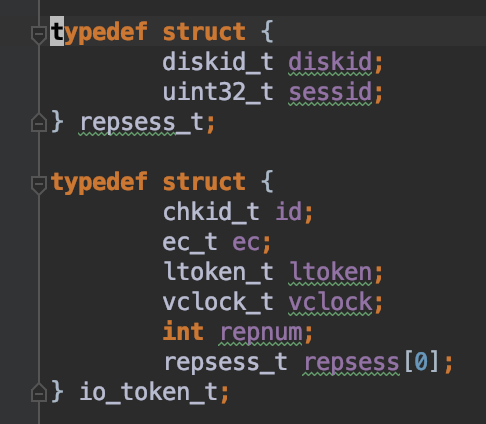
\includegraphics{../imgs/token.png}
\end{center}

range ctl和mds都在hash ring上。都采用了hash机制来定位目标节点。
所以\hl{有两个hash ring:range ctl和mds}。两个ring都通过mds master来维护。
ring的节点结构是什么?node and core?
\begin{center}
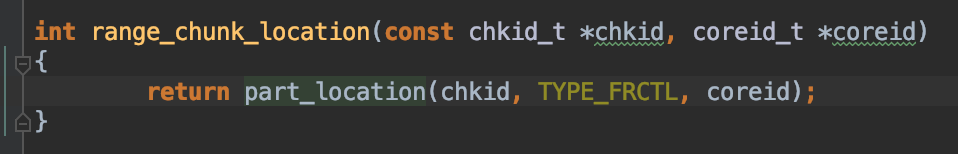
\includegraphics[width=11cm]{../imgs/chunk-location.png}
\end{center}

partition是range ctl和mdctl共用模块。range ctl目前归属frctl。

lease机制目前没用,如果需要把range ctl放置到session所在的位置(一个volume的所有range都在一个节点上?),
可以选用lease机制,而不用dht机制。怎么理解session?

一旦ring结构发生变化,会有什么影响?SSAN通过epoch来管理ring结构的变化。

ring上节点负载均匀性如何?

ring lock有什么用?在mds master上维护状态,处理ring发生变更的情况。
是否可通过引入epoch实现同样的功能?

GFM?解决全局同一视图的问题。

如何识别和处理stale消息?

\subsection{MDCTL}

hash ring上有一个节点充当master角色。如何选主,如何保持其唯一性?
通过etcd lock实现。

\subsection{BACTL}

diskid是全局的,在etcd上有目录。

\subsection{Driver}

diskmd磁盘访问接口,支持libnvme驱动。

需要管理物理内存,如hugepage和memory pool。

NVMe/RDMA需要访问物理内存。

\section{资源}

从\hl{资源的生命周期模型}开始思考。资源包括:\hl{集群、节点、core、磁盘、pool、volume、snapshot}等,以及内部资源。

ERD

\subsection{Cluster}

\subsection{Node}

Node是Process、Core、Disk等资源的合集。利用Core的方式是个亮点。

增删节点是重大事件

\subsection{Disk}

Disk导出,分配过程可以进行全局调度。

调度器位于md ctl。md ctl负责管理chkid到disk id的映射关系。
\todo{diskid类型}diskid采用16bit整数是否太小?

diskmap.c,不宜放入bactl。bactl所有API都带diskid,针对单盘进行。

怎么做到每个副本属于不同的节点的呢?

如何管理diskmap的版本呢?

\hl{数据分布的均匀性}: 节点和磁盘两种粒度

tier and cache?

负载均衡

\subsection{Pool}

\subsection{Volume}

\begin{enumbox}
\item TP
\item Recovery
\item Balance
\item QoS
\item ***
\item EC
\item Dedup
\item Compress
\item ***
\item RC
\end{enumbox}

\subsection{Snapshot}

如何共享底层对象?

consistency group

分析各种操作的复杂度,包括空间和时间。

\hrulefill

平安科技:可写快照

与COW平列实现ROW?

快照占据底层volume空间共享?

COW的问题
\begin{enumbox}
\item 影响写性能
\item Rollback慢
\item clone卷慢,scan snap tree。snapshot也可执行flatten
\end{enumbox}

snap头包含什么指针?

快照卷与物理卷什么对应关系,

映射表的管理粒度,是chunk还是page?范围,是全局还是私有?

COW一次读,两次写

ROW一次读,一次写

\hrulefill

SSAN的snapshot实现。

ROW,两层元数据?

vol id发生变化,凡是依赖于vol id的都需要进行适配。

\section{数据}

\subsection{ETCD}

\subsection{卷的元数据}

两层元数据,etcd指向顶层对象。每个对象属于一个卷,
因为不是一般的对象系统,\hl{在快照的情况下,无法直接共享}。

\chapter{快照和克隆}

\chapter{测试}

\lstset{numbers=left,
    frame=shadowbox,
    numberstyle= \tiny,
    keywordstyle= \color{ blue!70},commentstyle=\color{red!50!green!50!blue!50}, 
    rulesepcolor= \color{ red!20!green!20!blue!20} 
}

\section{已知问题}

\begin{enumbox}
\item vol resize会产生死锁
\item vol copy的提示
\item flat后保护快照
\end{enumbox}

\section{部署}

基本步骤:
\begin{enumbox}
\item 创建集群
\item 创建存储池
\item 向存储池添加磁盘(Tier, SSD Cache)
\item 创建卷
\item 创建快照
\end{enumbox}

\subsection{创建集群}

\begin{lstlisting}[language=bash]
lich prep t151 t152 t153
lich create t151 t152 t153
\end{lstlisting}

\hl{注意事项}:
\begin{compactenum}
\item 检查IP是否重复
\item 检查子网mask是否匹配
\item ...
\end{compactenum}

\subsection{创建存储池}

\begin{lstlisting}[language=bash]
lichbd pool create p1
\end{lstlisting}

\subsection{向存储池添加磁盘}

\begin{lstlisting}[language=bash]
lich.node --disk_add all --force --pool p1
\end{lstlisting}

\hl{注意事项}:
\begin{compactenum}
\item 存储池内每个节点上需要有SSD,支持tier功能
\item 存储池内每个节点上需要有SSD,支持SSD cache功能
\end{compactenum}

\subsection{创建卷}

\begin{lstlisting}[language=bash]
# 卷路径规范:<pool>/<protocol>/<volume>
# 三副本
# row2格式
lichbd vol create p1/iscsi/v1 --size 4096Gi --repnum 3 -F row2
lich.inspect --localize /iscsi/v1 0 --pool p1
\end{lstlisting}

\hl{注意事项}:
\begin{compactenum}
\item 卷格式:row2 or raw (default)
\item 三副本 (default: 2)
\item 关闭localize
\end{compactenum}

\subsection{创建快照}

\begin{lstlisting}[language=bash]
# 快照路径规范:<pool>/<protocol>/<volume>@<snap>
lichbd snap create p1/iscsi/v1@snap1
\end{lstlisting}

\section{工具}

省略...

\begin{lstlisting}[language=bash]
iscsiadm -m discovery -t st -p 192.168.251.202
\end{lstlisting}

\section{故障测试}

每类节点故障行为不同。除选举过程外,还有vip,iscsi连接,controller的切换,lease,io,恢复过程等。
评价可靠性的指标,主要是vdbench测试中,各种故障条件下io无中断。

另外,故障点还会破坏事务执行的原子性,如allocte过程,创建snapshot过程,
导致严重后果,如造成垃圾,数据状态不一致。如何通过可重入性,或事务解决此类问题?

快照的rollback,delete,flat都设计为可重入过程。如果任务执行失败,可以重新调度。
各种持久化状态之间,保持一致性。

\subsection{单磁盘故障}

磁盘有两种角色:数据盘和cache盘。拔cache盘等同于节点故障?

\subsection{节点故障}

节点有多种角色:
\begin{compactenum}
\item etcd master
\item lich admin
\item lich normal
\end{compactenum}

受VIP机制影响,arp协议会影响客户端到iscsi target的网络连接。
需要注意的是,大部分网络会禁用arp广播,单播则可以。

控制器的加载,lease获取等需要一定时间。

\chapter{项目}

PM的质量三角
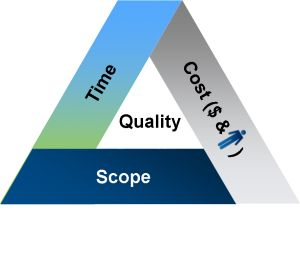
\includegraphics[width=8cm]{../imgs/quality.jpeg}

\section{范围}

道法自然

奥卡姆剃刀

滚雪球,定义MVP:
\begin{enumbox}
\item \hl{定义存储引擎},用各项特性对设计进行压力测试
\item CRC分析,明确职责,划分模块、定义接口
\item 尽快验证性能、一致性和可靠性
\item TDD 完善自动化测试
\item ***
\item Storage Driver
\item MM
\item ***
\item EC
\item Snapshot
\item Consistency Group
\end{enumbox}

\section{成本}

\section{时间}

行百里者半九十

群起而攻之

\chapter{MISC}

\section{GIT}

\begin{lstlisting}[language=bash,frame=single]
\item git remote add upstream http://gitlab.taocloud.com/suzaku2019/suzaku.git
\item git pull upstream master (将suzaku2019的内容更新到我本地)
\item git add .
\item git commit -m "desc"
\item git push origin master
\end{lstlisting}

\section{Hosts}

%\chapter{一致性}

\section{原理}

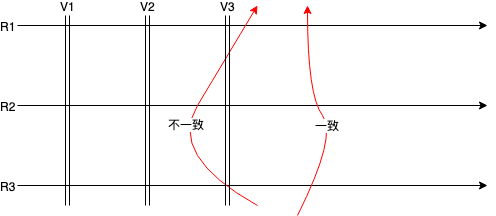
\includegraphics[width=11cm]{../imgs/consistency-splice.png}

从逻辑上讲,一致性是由任一对象的变更历史决定的。强一致性要求:
\begin{enumbox}
\item 任一对象的多个副本/分片,可以看作有限状态机,须按同一顺序执行变更。变更通常包括写IO和内部修复IO。
\item 已提交的写不能丢失
\item 能读到最新数据
\end{enumbox}

相比于副本机制,EC的各分片具有严格顺序。

从实现机制上来看,副本或EC的一致性,需要从\hl{对象版本、控制器和日志}几个方面来考虑。

恢复过程的关键是\hl{选择到正确的副本/分片}。分为几种情况:
\begin{enumbox}
\item EC的节点故障
\item EC的磁盘故障
\item 副本
\end{enumbox}

\section{副本一致性}

现象:观察到恢复完成后,有时vdi对象并不一致。

\todo{副本一致性}目前副本的一致性实现,机制上恐有问题。
恢复的选择步骤,各个副本独立运行选择过程,所依据的并非该对象各个副本的全局信息,而是相当局部的信息。
并不能保证一定选择到正确副本。

需要参考EC一致性的机制,选出primary协调IO和recovery活动。
副本的选择步骤相对简单:可用的最大版本的副本,以之为权威副本,覆盖其余。

\section{EC一致性}

\subsection{对象版本}

从概念上来说,SSAN按epoch组织对象,节点故障时提升epoch,磁盘故障时epoch不变,
通过强制升级epoch来模拟节点/磁盘混合故障。

epoch是集群级别的版本,epoch内节点成员关系不变。在SSAN实现里epoch被用作粗粒度的对象版本。

\subsection{控制器}

IO控制器是gateway,SSAN原始实现无恢复控制器,后针对任一对象引入primary数据分片作为恢复控制器。
这样就形成\hl{IO和恢复的双控架构},为了对象一致性,需要同步IO控制器和恢复控制器。

\subsection{日志}

无日志,难以处理特定情况下的恢复问题。比如4+2时,如果成功写入3个数据分片,则过程无法重入,无法
从该不一致状态修复到一致性状态。\hl{对条带对齐的IO,可采用REDO日志replay这个过程}。
维护UNDO日志则相对复杂。

\subsection{对象组织及其cache}
\label{subsec:object-dir}

因为可能在工作目录创建不同epoch的对象,工作目录下的对象名字也要包括epoch。

进一步可以考虑按epoch组织目录,这样可以简化关键操作,比如消除rename和link操作。
磁盘故障时,因为不升级epoch,所以需要特别处理,\hl{校正对象的磁盘位置,但不需要link了}。
需要保证过程的原子性。

维护磁盘对象结构的内存cache,在其上面提供API,合并stale cache和object list cache。
需要实现的API包括:
\begin{enumbox}
\item get\_obj\_list,获取一节点上所有对象的oid
\item get\_obj\_history,获取一个object的历史版本
\item get\_obj\_history2,获取一个object的历史版本,wd==0
\item stale\_cache\_compact,清除无效磁盘相关的记录
\end{enumbox}

\subsection{恢复实例}

恢复实例可以看作有限状态机。在恢复期间,SSAN进程运行一个恢复实例。
如果有新的故障,则执行上下文切换,切换到下一恢复实例。需要保证切换恢复实例过程的正确性。
任一时刻,最多有一个恢复实例在运行。

恢复状态机的每步转换都要满足safety和liveness条件,特别需要注意的是:
\begin{enumbox}
\item update epoch过程务必成功执行
\item 若一节点收不到recover peer,无法进入NOTIFY STANDBY DONE状态
\end{enumbox}

\subsection{TODO}

\begin{enumbox}
\item prepare object list,接收到非法oid
\item do\_event\_loop里ei->name出现乱码
\end{enumbox}

\section{EC一致性的改进之处}

具体见git仓库的提交日志。

\subsection{增强系统可追踪性}

主要通过日志机制来实现。把每个对象、io、恢复实例等等实体看作对象,追踪其生命周期行为,便于分析异常现象。

引入GOTO、SD\_ASSERT macro。

引入COREDUMP

引入RAMDISK

\subsection{create and write采用sync模式}

出现虽然写成功,后来发现对象内容为全零的情况。

\subsection{优化oidlist的索引}

优先修复vdi object。

采用bitmap检索data object和ledger object。\todo{摘除优先修复对象}\hl{数据量大时,优先修复的oid依然效率低}。

\subsection{改进对象组织方式}

参考小节~\ref{subsec:object-dir}

\subsection{改进stale object cache}

改进stale object cache模块,用于追踪对象在磁盘上的分布,可以理解为磁盘目录结构的cache。
通过支持所需API,来替代原来的object list cache和stale cache。同时也方便stale object的GC过程。

\subsection{恢复状态机引入新状态}

重构恢复实例的状态机。

引入RW\_INIT:为了实现没有进入prepare状态的恢复实例,可以切换到下一实例。一旦进入prepare阶段,则切换过程有所不同。
\hl{通用原则是确保rinfo上下文信息的安全性}。在有引用计数的情况下,不能被free掉。

引入RW\_UPDATE\_EPOCH:因为update epoch执行时间过长,为了不堵塞main线程,须放到工作线程中去做。

引入RW\_NOTIFY\_STANDBY\_DONE:放入同步点,以确保object list cache准备妥当,才能保证后续prepare object list过程无误。

避免prepare object list重复入队,导致修复崩溃

\subsection{磁盘空间不足时的恢复过程}

\todo{磁盘空间不足时的恢复过程}可以在finish object list过程,加入检查逻辑。检查项:
\begin{enumbox}
\item 每个disk的容量是否够用(执行hash运算后分布到该磁盘上的对象)
\item 对象的历史版本可能没及时回收
\item 在恢复过程中会有新的create and write
\end{enumbox}

如果不能通过检查,则标记节点状态为NODE\_NOSPC,影响到的操作:
\begin{enumbox}
\item 读写io
\item 退出恢复过程
\end{enumbox}

在此状态下,运行执行删除卷操作,以回收空间。回收完成后,重新进入修复状态。

\subsection{retry机制}

retry机制的使用需要具体分析,内部过程慎用retry,避免堵塞main线程,使系统失去响应能力。

重试次数和timeout值的选择也影响到故障切换时长和IO中断时长。

\subsection{Too many open files}

文件句柄数量控制,由最大1024改为1048576。直接在SSAN进程内设定。

\subsection{scli cluster check的OOM现象}

因为check过程相对低效,导致等待check的队列大量积压,消耗大量内存,引起OOM。
故引入QoS机制,限制队列长度,减少内存消耗。

\subsection{日志缓冲区设定过小,导致日志丢失}

\section{小结}

指导原则
\begin{enumbox}
\item 一致性问题要对标相关参考模型
\item 采用流体动力学模型分析性能瓶颈
\item 工欲善其事必先利其器
\end{enumbox}

工具方面
\begin{enumbox}
\item 完整日志追踪系统,细粒度地追踪程序运行时行为
\item 加入PROFILE日志,辅助分析各个过程的性能特征
\item 多用断言,以捕获程序中的不变式,尽早暴露问题
\item 生成COREDUMP
\item 采用valgrind分析内存问题
\item 采用egrep分析日志,保留相关日志的相对顺序
\item 采用fio的verify和scli cluster check机制验证一致性
\item ***
\item 尽量保障开发和测试环境
\end{enumbox}

egrep的使用示例:
\begin{lstlisting}[language=bash,frame=single]
egrep 'start_recovery|free_recovery_info' ssan.log
egrep 'start_recovery|iops' ssan.log
\end{lstlisting}

关于日志子系统,需要从内容和形式上进一步规范化。
\begin{enumbox}
\item 可动态调整日志等级
\item 管理对象的生命周期活动
\item 捕获尽可能多的上下文信息
\item 提高日志的信息密度
\item 关键字
\end{enumbox}

性能分析
\begin{enumbox}
\item 流出等于流入
\item 下游处理能力大于流入流量
\item 调度能力大于下游处理能力
\end{enumbox}

重点是提升下游节点的处理能力和中间节点的调度能力。
以修复为例,下游处理能力对应恢复性能,调度能力对应main线程的调度能力。

\section{suazku一致性方案}

epoch down set

GFM

\subsection{IO流程}

\mygraphics{../imgs/rangectl/rep-sessid.png}

\mygraphics{../imgs/rangectl/io-token.png}

降级模式,只有降级模式下才需要序列化clock?

\subsection{一致性的判断条件}

clock全等(skip dirty==1)。如果不等,则选取最大的,覆盖其余。

\subsection{故障检测机制}

查询rangectl以确定是否需要恢复?

\subsection{如何选出权威副本}

\mygraphics{../imgs/rangectl/ABA.png}

ceph用up\_thru,也可以反方向标记stale,只是代价较高。

如何识别在B期间是否有更新操作?

\subsection{恢复过程}

恢复是独立于core线程的外部线程,卷怎么映射到各个恢复线程上?

open并scan卷。

\subsection{多点写}

\mygraphics{../imgs/rangectl/multipoint-write.png}

先分析单点写,再扩展到多点写的情况。

本质问题是什么?

这种现象并不是多点写特有的,在最简单的情况下,单点写入,如果\hl{频繁断开initiator和target之间的网络},也有可能发生数据破坏的现象。
\hl{新的session已有一个或多个io写入,又收到了stale session发来的io},如果不拒绝的话,就会破坏数据。

leader最多只有一个,而session可以有一个或多个,无法分辨哪个是stale的?
session3要替代session2,而session 1要长期共存。所以不能简单地通过response进行分辨。

新session与旧session存在两种关系:
\begin{myeasylist}{itemize}
& 替代
& 共存
\end{myeasylist}

end-to-end的验证机制。

再次开启新session,session id会变吗?如何区分新旧session发出的io,包括flying io message?
session version的语义是代表了一个卷的连接结构的变化。epoch代表了集群级故障信息的变化。

tgt收到ESTALE时,drop it。依赖于上层app的timeout \hl{retry机制}。
tgt周期性地poll该值,主动更新,可以减少ESTALE。

在bactl上维护每个chunk看到的最新session version,规则:
\begin{myeasylist}{itemize}
& io.sversion < chunk.sversion, return ESTALE
& io.sversion > chunk.sversion, let chunk.sversion = io.sversion
\end{myeasylist}

稳定运行时,两者相等。有新session生成时,且已到达过bactl,所有持有较小sversion的io都会被标记为ESTALE。

怎么区分正常session和过期session,两者都可能小于当前最大session version。

新session会影响到所有已存在的session,包括正常工作的和发生故障的,如何降低该影响?

在此基础上,epoch和clock机制如何发挥作用?若一session退出,导致clock不连续

与redirect的关系?

NVMf的error handling机制如何?

\hrulefill

\mygraphics{../imgs/kb/raft-stale-leader.png}

RAFT的term跟踪的是leader的变化历史,消息是leader发出的。io携带term,可以识别stale leader。

sversion跟踪的是session的变化历史。

%\chapter{性能}

从宏观到微观

\section{设计原则}

\mygraphicsh{../imgs/arch/perf-options.png}

\begin{myeasylist}{itemize}
& 平衡性
& 局部性
& 并行性
\end{myeasylist}

优化项
\begin{myeasylist}{itemize}
& log
& O3
& IO FUNC
& inline
& likely
& HUGEPAGE
& cacheline
& irq
& unlock ring
& get token
& SPDK
&& driver
&& target
\end{myeasylist}

\section{怎么分析单卷性能}

\mygraphicsh{../imgs/io-path.png}

\section{资源}

\subsection{CPU}

\subsection{内存}

hugepage

\subsection{磁盘}

libnvme

\subsection{网络}

\begin{enumbox}
\item TCP
\item RDMA
\end{enumbox}

\section{Target}

\begin{enumbox}
\item iSCSI
\item iSER
\item NVMf
\end{enumbox}

\section{Multi Path}


\end{document}
